\chapter{Синглет, неравенство Белла и запрет клонирования}

\lectureoverview{Относительный знак минус превращает просто коррелированное состояние двух спинов в инвариантный относительно вращений синглет. Мы отождествляем это состояние, вычисляя его полный спин, используем его совершенную антикорреляцию для постановки эксперимента Белла и переводим классические высказывания в квантовые операторы-проекторы. Получающиеся вероятности нарушают классическое неравенство Белла, получаемое подсчётом. Затем вопросы о локальности, временном порядке эксперимента и неопределённости приводят ко второму следствию линейной квантовой механики: неизвестное состояние нельзя скопировать универсальной клонирующей машиной.}

\section{Какую разницу может дать один знак?}

Рассмотрим два электрона и опустим символ тензорного произведения в базисных состояниях:
\begin{equation}
  \ket{ud}\equiv\ket{u}_1\otimes\ket{d}_2,
  \qquad
  \ket{du}\equiv\ket{d}_1\otimes\ket{u}_2.
\end{equation}
Две особенно простые суперпозиции различаются только одним знаком,
\begin{equation}
  \ket{\psi_\pm}
  =
  \frac{\ket{ud}\pm\ket{du}}{\sqrt2}.
  \label{eq:l05-two-signs}
\end{equation}
Множитель \(1/\sqrt2\) делает полную вероятность равной единице. В любом из этих состояний измерение вдоль третьей оси даёт противоположные ответы: если у электрона 1 спин направлен вверх, то у электрона 2 спин направлен вниз, и наоборот. Поэтому по одной лишь этой корреляции знак обнаружить нельзя. Тем не менее эти два состояния физически различны.

В вычислениях мы многократно будем использовать действие операторов Паули
\begin{align}
  \sigma_1\ket{u}&=\ket{d},&
  \sigma_1\ket{d}&=\ket{u},\nonumber\\
  \sigma_2\ket{u}&=i\ket{d},&
  \sigma_2\ket{d}&=-i\ket{u},\nonumber\\
  \sigma_3\ket{u}&=\ket{u},&
  \sigma_3\ket{d}&=-\ket{d}.
  \label{eq:l05-pauli-actions}
\end{align}
Обозначение \(\sigma_i\) мы резервируем для операторов, действующих на электрон 1, и вводим такое же семейство \(\tau_i\), действующее на электрон 2.

\begin{figure}[htbp]
\centering
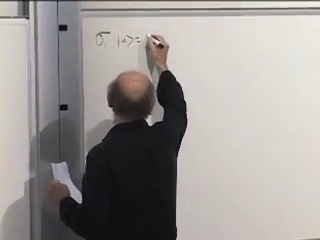
\includegraphics[width=0.62\linewidth]{lecture_05_figure_02.png}
\caption{Полная таблица действия операторов Паули, используемая на протяжении всего сравнения.}
\lectureframe{00:03:15}
\end{figure}

Ни у одного из составляющих спинов ни в одном из этих состояний нет предпочтительного направления:
\begin{equation}
  \expect{\sigma_i}_{\psi_\pm}=0,
  \qquad
  \expect{\tau_i}_{\psi_\pm}=0,
  \qquad i=1,2,3.
  \label{eq:l05-local-zero}
\end{equation}
Например, явная проверка, запрошенная для плюсового состояния, даёт
\begin{align}
  \bra{\psi_+}\sigma_3\ket{\psi_+}
  &=
  \frac12
  \bigl(\bra{ud}+\bra{du}\bigr)
  \bigl(\ket{ud}-\ket{du}\bigr)\nonumber\\
  &=
  \frac12(1-1)=0.
  \label{eq:l05-sigma3-expectation}
\end{align}
Перекрёстные члены исчезают, потому что \(\braket{ud}{du}=0\).

\begin{figure}[htbp]
\centering
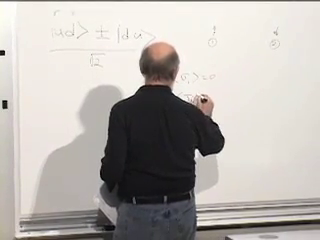
\includegraphics[width=0.78\linewidth]{lecture_05_figure_03.png}
\caption{Среднее значение для плюсового состояния вычисляется, если подействовать \(\sigma_3\) и воспользоваться ортогональностью.}
\lectureframe{00:07:00}
\end{figure}

\begin{classroomqa}
\lecturetimestamp{00:07:13}
\audiencequestion{Означает ли нулевое среднее значение, что при измерении одного спина можно получить значение нуль?}
\lecturerresponse{Нет. У компоненты одного спина возможны только результаты \(+1\) и \(-1\); у \(\sigma_i\) нет собственного значения, равного нулю. Уравнение~\eqref{eq:l05-local-zero} говорит, что при многократных измерениях получается равновероятное подбрасывание честной монеты, а не то, что какой-то отдельный результат равен нулю.}
\end{classroomqa}

Таким образом, первый правдоподобный диагностический признак не сработал. Локальные средние не чувствуют относительного знака, поэтому нужно измерять свойство пары.

\section{Полный спин выделяет синглет}

Магнитный момент пары представляется векторной суммой
\begin{equation}
  \boldsymbol{\Sigma}
  =
  \boldsymbol{\sigma}+\boldsymbol{\tau}.
\end{equation}
Его третья компонента аннулирует оба базисных вектора:
\begin{align}
  (\sigma_3+\tau_3)\ket{ud}
  &=(1-1)\ket{ud}=0,\nonumber\\
  (\sigma_3+\tau_3)\ket{du}
  &=(-1+1)\ket{du}=0.
\end{align}
Следовательно,
\begin{equation}
  (\sigma_3+\tau_3)\ket{\psi_\pm}=0.
\end{equation}
Для обоих выборов знака полная третья компонента в каждом отдельном опыте равна нулю.

Первая компонента их различает. Из уравнения~\eqref{eq:l05-pauli-actions},
\begin{align}
  (\sigma_1+\tau_1)\ket{ud}
  &=\ket{dd}+\ket{uu},\nonumber\\
  (\sigma_1+\tau_1)\ket{du}
  &=\ket{uu}+\ket{dd}.
\end{align}
Следовательно,
\begin{align}
  (\sigma_1+\tau_1)\ket{\psi_+}
  &=
  \sqrt2\bigl(\ket{uu}+\ket{dd}\bigr),\nonumber\\
  (\sigma_1+\tau_1)\ket{\psi_-}
  &=0.
  \label{eq:l05-total-x}
\end{align}
У плюсового состояния среднее значение этой наблюдаемой может быть нулевым, но собственным состоянием этой наблюдаемой с собственным значением нуль оно не является.

\begin{classroomqa}
\lecturetimestamp{00:13:02}
\audiencequestion{Какие результаты может давать полная компонента, когда состояние ею не аннулируется?}
\lecturerresponse{У каждой составляющей ответ равен \(+1\) или \(-1\), так что их сумма может быть \(2\), \(0\) или \(-2\). Нулевое среднее значение не вынуждает получать нуль в каждом отдельном опыте.}
\end{classroomqa}

Вторая компонента завершает проверку. Её множители \(i\) сокращаются в антисимметричной комбинации:
\begin{equation}
  (\sigma_2+\tau_2)\ket{\psi_-}=0.
\end{equation}
Поэтому все три компоненты аннулируют минусовое состояние,
\begin{equation}
  \bigl(\boldsymbol{\sigma}+\boldsymbol{\tau}\bigr)
  \cdot\hat n\,\ket{\psi_-}=0
  \qquad\text{for every unit vector }\hat n.
  \label{eq:l05-singlet-any-axis}
\end{equation}

\begin{figure}[htbp]
\centering
\includegraphics[width=0.84\linewidth]{lecture_05_figure_06.png}
\caption{Покомпонентные сокращения, показывающие, что минусовое состояние имеет полный спин нуль.}
\lectureframe{00:16:30}
\end{figure}

Антисимметричное состояние \(\ket{\psi_-}\) — это \emph{синглет}. Оно инвариантно относительно вращений: каждая ось даёт один и тот же ответ для полного спина, нуль. Симметричное состояние из уравнения~\eqref{eq:l05-two-signs} принадлежит триплетному сектору.

\begin{classroomqa}
\lecturetimestamp{00:19:06}
\audiencequestion{Верно ли утверждение о противоположных спинах только в среднем?}
\lecturerresponse{Для синглета это верно в каждом отдельном опыте. Уравнение~\eqref{eq:l05-singlet-any-axis} является уравнением на собственный вектор, поэтому измерение одной и той же компоненты у обеих частиц всегда даёт ответы, сумма которых равна собственному значению нуль.}
\end{classroomqa}

\begin{classroomqa}
\lecturetimestamp{00:19:36}
\audiencequestion{Почему другое состояние называется триплетом?}
\lecturerresponse{Это название происходит от трёх состояний в мультиплете с полным спином один. Его вывод откладывается; для настоящего вычисления нужен лишь контраст между симметричным состоянием и одномерным синглетным сектором.}
\end{classroomqa}

Если Боб измеряет любую компоненту спина своего электрона, он сразу знает, что получила бы Алиса, измерив ту же компоненту у своего: её ответ должен быть противоположным. Это корреляция Эйнштейна--Подольского--Розена. Пара скрытых монет тоже может нести противоположные результаты, но только для одного заранее оговорённого вопроса. Синглет даёт совершенную антикорреляцию для любой выбранной пространственной оси.

\begin{classroomqa}
\lecturetimestamp{00:20:55}
\audiencequestion{Эйнштейн, Подольский и Розен первыми обнаружили запутанность?}
\lecturerresponse{Нет. Шрёдингер обсуждал это явление и ввёл язык запутанности. Аргумент EPR особенно резко поставил проблему дальних корреляций.}
\end{classroomqa}

\begin{classroomqa}
\lecturetimestamp{00:23:50}
\audiencequestion{Нарушает ли немедленная корреляция причинность, и имеет ли значение, кто из наблюдателей измеряет первым?}
\lecturerresponse{Нет. Никакое пригодное для использования сообщение не передаётся. Локальные результаты Алисы остаются равновероятными независимо от того, измеряет Боб или нет, при любом инерциальном порядке событий. Проверить корреляцию она может только после того, как получит результат Боба по обычному классическому каналу, который не может обогнать свет.}
\end{classroomqa}

\section{Неравенство Белла — это классический подсчёт}

Статус результата Белла может казаться неустойчивым. В одни дни он выглядит глубочайшей чертой квантовой механики; в другие — ещё одним неизбежным следствием формализма. И сам Белл, и Фейнман тоже могли выражать оба этих отношения. Однако само неравенство элементарно. Неожиданность состоит в его нарушении.

Рассмотрим обычное множество объектов. Каждый объект может обладать или не обладать тремя свойствами \(A\), \(B\) и \(C\). Пусть \(N(A,\neg B)\) обозначает число объектов, которые имеют \(A\), но не \(B\). Классическая логика множеств влечёт
\begin{equation}
  N(A,\neg B)+N(B,\neg C)
  \geq
  N(A,\neg C).
  \label{eq:l05-bell-count}
\end{equation}
Доказательством служит включение множеств
\begin{equation}
  A\cap C^{c}
  \subseteq
  (A\cap B^{c})\cup(B\cap C^{c}).
  \label{eq:l05-set-inclusion}
\end{equation}
В самом деле, элемент \(A\cap C^c\) либо принадлежит \(B\), либо нет. В первом случае он принадлежит \(B\cap C^c\); во втором — \(A\cap B^c\). При подсчёте объединения множество слева можно только пересчитать с избытком.

\begin{figure}[htbp]
\centering
\includegraphics[width=0.78\linewidth]{lecture_05_figure_07.png}
\caption{Доказательство на доске разбивает три перекрывающихся классических подмножества на области с неотрицательными числами.}
\lectureframe{00:31:15}
\end{figure}

Эквивалентно, обозначьте непересекающиеся области диаграммы трёх множеств неотрицательными целыми числами \(N_i\). Обе части уравнения~\eqref{eq:l05-bell-count} содержат области, соответствующие \(A\cap C^c\), тогда как левая часть содержит дополнительные неотрицательные области. Ничего квантового здесь ещё не появилось. Это теорема о подмножествах и обычных логических альтернативах.

\section{Преобразование утверждения о множествах в спиновый эксперимент}

Приготовим много независимых электронных пар в синглетном состоянии и определим три высказывания об электроне 1:
\begin{align}
  A&:\ \text{spin 1 is up at }0^\circ\text{, along the third axis},\nonumber\\
  B&:\ \text{spin 1 is up at }45^\circ\text{ in the }zx\text{-plane},\nonumber\\
  C&:\ \text{spin 1 is up at }90^\circ\text{, along the first axis}.
  \label{eq:l05-abc}
\end{align}

\begin{figure}[htbp]
\centering
\includegraphics[width=0.82\linewidth]{lecture_05_figure_08.png}
\caption{Три спиновых высказывания заданы при \(0^\circ\), \(45^\circ\) и \(90^\circ\) в одной плоскости.}
\lectureframe{00:39:00}
\end{figure}

В синглете отрицание высказывания об электроне 1 можно переписать как положительное высказывание об электроне 2. Например,
\begin{align}
  \neg B
  &:\ \text{spin 1 is down at }45^\circ\nonumber\\
  &\Longleftrightarrow
  \text{spin 2 is up at }45^\circ.
\end{align}
Аналогично, \(\neg C\) превращается в утверждение, что у электрона 2 спин направлен вверх при \(90^\circ\).

\begin{classroomqa}
\lecturetimestamp{00:40:04}
\audiencequestion{Должно ли \(\neg C\) означать, что у электрона 2 спин направлен вниз при \(90^\circ\)?}
\lecturerresponse{Нет. Сначала нужно отрицать \(C\): у электрона 1 спин направлен вниз при \(90^\circ\). Затем совершенная антикорреляция синглета означает, что у электрона 2 спин направлен вверх вдоль той же оси. Эти два обращения нужно держать раздельно.}
\end{classroomqa}

Для большого ансамбля числа событий и вероятности различаются только общим числом приготовленных пар. Инвариантность относительно вращений также даёт
\begin{equation}
  P(A,\neg B)=P(B,\neg C),
\end{equation}
потому что второй эксперимент получается из первого поворотом на \(45^\circ\). Поэтому классическое неравенство Белла потребовало бы
\begin{equation}
  2P(A,\neg B)\geq P(A,\neg C).
  \label{eq:l05-bell-probability}
\end{equation}
Теперь нам нужен эффективный способ вычислить эти вероятности.

\section{Высказывания становятся проекторами}

В обычном трёхмерном векторном пространстве проектор устраняет всякую компоненту, перпендикулярную выбранному подпространству. Одномерный проектор ортогонально опускает вектор на прямую; двумерный — на плоскость. Если \(P\) проектирует на заданное подпространство,
\begin{equation}
  P\ket{\alpha}=\ket{\alpha_P}.
\end{equation}

\begin{figure}[htbp]
\centering
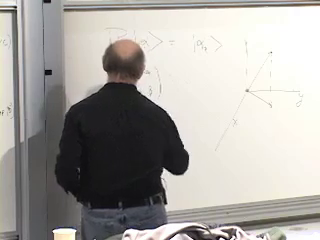
\includegraphics[width=0.76\linewidth]{lecture_05_figure_04.png}
\caption{Геометрическая проекция и её операторное обозначение вводятся параллельно.}
\lectureframe{00:49:53}
\end{figure}

\begin{figure}[htbp]
\centering
\begin{tikzpicture}[scale=1.05,>=Latex]
  \draw[->] (-0.25,0)--(4.0,0);
  \draw[thick] (-0.25,-0.25)--(3.55,2.6);
  \draw[->,very thick] (0,0)--(2.25,3.05)
    node[above] {\(\ket{\alpha}\)};
  \coordinate (P) at (2.72,1.98);
  \draw[dashed] (2.25,3.05)--(P);
  \draw[->,very thick] (0,0)--(P)
    node[right] {\(\ket{\alpha_P}\)};
  \node[below right] at (3.1,2.25) {projected subspace};
\end{tikzpicture}
\caption{Аккуратная реконструкция геометрии проекции.}
\end{figure}

В односпиновом гильбертовом пространстве высказыванию о том, что \(\sigma_3=+1\), соответствует одномерное подпространство, натянутое на \(\ket{u}\). Его проектор действует так
\begin{equation}
  P_{\sigma_3=+1}
  \begin{pmatrix}\alpha\\\beta\end{pmatrix}
  =
  \begin{pmatrix}\alpha\\0\end{pmatrix},
  \qquad
  P_{\sigma_3=-1}
  \begin{pmatrix}\alpha\\\beta\end{pmatrix}
  =
  \begin{pmatrix}0\\\beta\end{pmatrix}.
  \label{eq:l05-projector-actions}
\end{equation}

\begin{classroomqa}
\lecturetimestamp{00:49:55}
\audiencequestion{Показывает ли первый проектор, насколько высоко вектор поднимается по вертикальной оси?}
\lecturerresponse{Нет. Он просто отбрасывает ортогональный коэффициент \(\beta\). Эти компоненты — амплитуды в гильбертовом пространстве, а не обычные пространственные координаты спина.}
\end{classroomqa}

\begin{figure}[htbp]
\centering
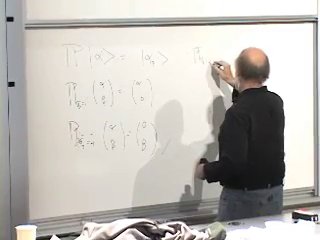
\includegraphics[width=0.78\linewidth]{lecture_05_figure_05.png}
\caption{Сначала проекторы действуют на произвольный спинор, а затем записываются в виде явных матриц.}
\lectureframe{00:51:40}
\end{figure}

Матричная форма имеет вид
\begin{equation}
  P_{\sigma_3=+1}
  =
  \begin{pmatrix}1&0\\0&0\end{pmatrix}
  =
  \frac{I+\sigma_3}{2}.
  \label{eq:l05-p3}
\end{equation}
Та же конструкция работает для любого единичного вектора \(\hat n\):
\begin{equation}
  P_{\boldsymbol{\sigma}\cdot\hat n=+1}
  =
  \frac{I+\boldsymbol{\sigma}\cdot\hat n}{2}.
  \label{eq:l05-pn}
\end{equation}

\begin{classroomqa}
\lecturetimestamp{00:53:09}
\audiencequestion{Каков проектор на \(\sigma_1=+1\)?}
\lecturerresponse{Замените \(\sigma_3\) на \(\sigma_1\) в уравнении~\eqref{eq:l05-p3}: \(P_{\sigma_1=+1}=(I+\sigma_1)/2\).}
\end{classroomqa}

Правило Борна теперь принимает полезную форму для высказываний:
\begin{equation}
  P(\mathcal A\text{ is true in }\ket{\psi})
  =
  \bra{\psi}P_{\mathcal A}\ket{\psi}.
  \label{eq:l05-projector-born}
\end{equation}
Для нормированного спинора \(\ket{\psi}=(\alpha,\beta)^T\) из уравнения~\eqref{eq:l05-projector-born} при \(P_{\sigma_3=+1}\) получается \(|\alpha|^2\), в точности как и должно быть.

Этот язык выявляет различие между классическими и квантовыми высказываниями. В классической логике свойству соответствует подмножество некоторого множества. В квантовой механике свойству соответствует подпространство гильбертова пространства или, что эквивалентно, его проектор. Подмножества и векторные подпространства не подчиняются одним и тем же операциям решётки; противоречие Белла вырастает из этого различия.

\subsection{Совместный проектор Белла}

Для \(A\wedge\neg B\) электрон 1 должен иметь спин вверх вдоль третьей оси, а электрон 2 — спин вверх вдоль
\begin{equation}
  \hat n_{45}=\frac{\hat x+\hat z}{\sqrt2}.
\end{equation}
Соответствующая компонента второго спина равна
\begin{equation}
  \boldsymbol{\tau}\cdot\hat n_{45}
  =
  \frac{\tau_1+\tau_3}{\sqrt2}.
\end{equation}
Следовательно, совместный проектор имеет вид
\begin{equation}
  P_{A\wedge\neg B}
  =
  \frac{I+\sigma_3}{2}
  \frac{I+(\tau_1+\tau_3)/\sqrt2}{2}.
  \label{eq:l05-joint-projector}
\end{equation}

\begin{classroomqa}
\lecturetimestamp{00:59:18}
\audiencequestion{Почему в спиновой компоненте при \(45^\circ\) стоит множитель \(1/\sqrt2\)?}
\lecturerresponse{Направление должно быть единичным вектором. Его компоненты по первой и третьей осям обе равны \(1/\sqrt2\), поэтому соответствующая наблюдаемая есть \((\tau_1+\tau_3)/\sqrt2\).}
\end{classroomqa}

\begin{classroomqa}
\lecturetimestamp{01:00:52}
\audiencequestion{Всё выражение \(I+\boldsymbol{\tau}\cdot\hat n_{45}\) делится на два?}
\lecturerresponse{Да. Проектор равен \(\bigl(I+\boldsymbol{\tau}\cdot\hat n_{45}\bigr)/2\); множитель \(1/2\) умножает весь числитель.}
\end{classroomqa}

Два множителя в уравнении~\eqref{eq:l05-joint-projector} действуют на разные тензорные сомножители и коммутируют. Их применение сначала удаляет всякую компоненту, в которой у электрона 1 спин вниз, а затем — всякую оставшуюся компоненту, в которой у электрона 2 спин вниз вдоль \(\hat n_{45}\).

\section{Квантовые числа обращают неравенство}

Пусть
\begin{equation}
  \ket{\psi_s}
  =
  \frac{\ket{ud}-\ket{du}}{\sqrt2}
\end{equation}
обозначает синглет. Начнём с
\begin{equation}
  P(A,\neg B)
  =
  \bra{\psi_s}P_{A\wedge\neg B}\ket{\psi_s}.
\end{equation}
Множитель \((I+\sigma_3)/2\) уничтожает \(\ket{du}\) и оставляет \(\ket{ud}/\sqrt2\). Второй множитель затем даёт
\begin{align}
  \frac{I+(\tau_1+\tau_3)/\sqrt2}{2}\ket{ud}
  &\notag\\[-0.3em]
  &=
  \frac12
  \left[
    \ket{ud}
    +\frac{\ket{uu}-\ket{ud}}{\sqrt2}
  \right]\nonumber\\
  &=
  \frac12
  \Biggl[
    \left(1-\frac1{\sqrt2}\right)\ket{ud}
  \nonumber\\
  &\qquad
    +\frac1{\sqrt2}\ket{uu}\Biggr].
  \label{eq:l05-projector-action}
\end{align}
Член \(\ket{uu}\) имеет нулевое перекрытие с бра-вектором синглета, а оставшиеся нормировочные множители дают
\begin{equation}
  P(A,\neg B)
  =
  \frac14\left(1-\frac1{\sqrt2}\right).
  \label{eq:l05-pab}
\end{equation}

\begin{figure}[htbp]
\centering
\includegraphics[width=0.88\linewidth]{lecture_05_figure_09.png}
\caption{При вычислении проектором сохраняется перекрытие с \(\ket{ud}\) и отбрасывается ортогональный вклад \(\ket{uu}\).}
\lectureframe{01:08:20}
\end{figure}

Инвариантность относительно вращений даёт тот же результат для следующей пары направлений:
\begin{equation}
  P(B,\neg C)
  =
  \frac14\left(1-\frac1{\sqrt2}\right).
\end{equation}
Для \(A\wedge\neg C\) второй осью является первая пространственная ось, поэтому
\begin{equation}
  P_{A\wedge\neg C}
  =
  \frac{I+\sigma_3}{2}\frac{I+\tau_1}{2}.
\end{equation}
Первый множитель снова оставляет \(\ket{ud}/\sqrt2\). Член с \(\tau_1\) даёт \(\ket{uu}\), которое ортогонально бра-вектору синглета, тогда как член с единичным оператором сохраняется. Следовательно,
\begin{equation}
  P(A,\neg C)=\frac14.
  \label{eq:l05-pac}
\end{equation}
Объединяя три результата,
\begin{equation}
  \underbrace{
  P(A,\neg B)+P(B,\neg C)
  }_{\frac12(1-1/\sqrt2)\approx0.146}
  <
  \underbrace{
  P(A,\neg C)
  }_{\frac14=0.25}.
  \label{eq:l05-bell-violation}
\end{equation}

\begin{figure}[htbp]
\centering
\includegraphics[width=0.84\linewidth]{lecture_05_figure_10.png}
\caption{На завершённом расчёте на доске показаны меньшая левая часть неравенства Белла и большая правая часть.}
\lectureframe{01:12:15}
\end{figure}

Уравнение~\eqref{eq:l05-bell-violation} обращает уравнение~\eqref{eq:l05-bell-probability}. Вывод не в том, что квантовая механика противоречит сама себе. Он в том, что синглетные корреляции не могут возникнуть из локальной классической модели, в которой все три высказывания о спине имеют обычные теоретико-множественные истинностные значения, не зависящие от удалённого выбора измерения. Классическая симуляция может воспроизвести корреляции, только отказавшись по меньшей мере от одного из белловских предположений, наиболее явно — от локальности.

\section{Что проверяет эксперимент Белла}

Квантовая механика уже предсказывает нарушение. Эксперимент должен дополнительно закрыть классическую лазейку, при которой один детектор сообщает другому, какую настройку или какой результат он получил. Два крыла установки должны быть достаточно далеко друг от друга, а выборы настроек и регистрации — достаточно близки по времени, чтобы световой сигнал не мог пройти между ними. Эксперимент Aspect убедительно реализовал на практике такие временные условия и такую изоляцию.

\begin{classroomqa}
\lecturetimestamp{01:13:15}
\audiencequestion{Если квантовая механика уже даёт ответ, научили ли нас чему-нибудь эксперименты Белла?}
\lecturerresponse{Они проверили, следует ли природа квантовому предсказанию именно в этом корреляционном эксперименте, и, что существенно, сделали два измерительных крыла независимыми в пределах соответствующего времени прохождения света. Сами по себе экспериментальный контроль и временная синхронизация были серьёзными достижениями.}
\end{classroomqa}

\begin{classroomqa}
\lecturetimestamp{01:18:19}
\audiencequestion{Что добавил Белл после эйнштейновского обсуждения жуткого действия на расстоянии?}
\lecturerresponse{Белл дал количественное неравенство. Он указал осуществимый корреляционный эксперимент, квантовое предсказание для которого исключает, что в основе лежит локальное классическое описание, вместо того чтобы оставлять возражение на уровне философского беспокойства. Сам Белл сохранял двойственное отношение к тому, является ли это неизбежным или глубоким, и со временем всё охотнее ставил под вопрос стандартную квантовую механику.}
\end{classroomqa}

Частицы могут находиться на расстоянии многих миль друг от друга и всё же оставаться в одном совместном состоянии, но это всё равно квантовый эксперимент над малыми системами. Взаимодействия с окружающей средой имеют тенденцию разрушать необходимые фазовые соотношения. Молекулы воздуха, посторонние фотоны и тепловые возмущения могут запутываться с парой, поэтому разнесение нужно проводить в холодной, хорошо изолированной среде.

\begin{classroomqa}
\lecturetimestamp{01:19:53}
\audiencequestion{Превращает ли общее состояние, простирающееся на большое расстояние, такую систему в макроскопический квантовый объект?}
\lecturerresponse{Лучше описывать это как малые квантовые системы, далеко разнесённые друг от друга. Расстояние между ними может быть большим, но сохранять их совместную волновую функцию становится всё труднее, потому что неконтролируемое взаимодействие с окружающей средой разрушает полезную когерентность. Два обычных шара для боулинга не реализуют тот же эксперимент.}
\end{classroomqa}

\begin{classroomqa}
\lecturetimestamp{01:21:23}
\audiencequestion{Может ли измерение одной частицы раскрыть комплементарную информацию о другой и тем самым обойти принцип неопределённости?}
\lecturerresponse{Можно измерить, например, положение одной частицы и импульс другой. Это не является одновременным измерением некоммутирующих наблюдаемых у одной частицы. Ограничение неопределённости для одной системы не было обойдено.}
\end{classroomqa}

\section{Когда произведение означает «и»?}

В вычислении Белла перемножались два проектора. Это представляет конъюнкцию только для совместимых высказываний.

\begin{classroomqa}
\lecturetimestamp{01:22:39}
\audiencequestion{Почему произведение двух проекторов представляло логическое слово «и»?}
\lecturerresponse{Потому что эти два проектора коммутируют. Один действует на электрон 1, а другой — на электрон 2, поэтому их порядок несущественен и оба свойства можно проверять совместно. Для одного электрона \((I+\sigma_3)/2\) и \((I+\sigma_1)/2\) не коммутируют; спин вверх вдоль обеих осей не является совместно определённым высказыванием такого рода.}
\end{classroomqa}

Это ещё одно место, где квантовые высказывания расходятся с обычными подмножествами. Классическое пересечение существует всегда. Квантовый аналог, представляемый произведением проекторов, имеет предполагаемый логический смысл только тогда, когда соответствующие подпространства совместимы.

То же обсуждение подводит и к самому измерению. У измерительного прибора есть состояние указателя. Если электрон со спином вверх переводит указатель в одно положение, а со спином вниз — в другое, то электрон в суперпозиции запутывается с двумя положениями указателя. Поэтому измерение можно изучать как запутывание между системой и аппаратом. Эту проблему мы пока откладываем в пользу более короткой теоремы, использующей только линейность.

\begin{classroomqa}
\lecturetimestamp{01:25:09}
\audiencequestion{Полезно ли рассматривать коллапс волновой функции как то, что одно измерение накладывает ограничение на совместное состояние?}
\lecturerresponse{Этот вопрос относится к процессу измерения. Прибор и измеряемая система запутываются: одно значение спина коррелирует с одним положением указателя, а другое значение — с другим. Подробное обсуждение измерения отложено.}
\end{classroomqa}

\section{Линейность запрещает универсальный ксерокс}

Нужен только один факт о временной эволюции. Если физический процесс осуществляет преобразование
\begin{equation}
  \ket{a}\longrightarrow\ket{a'},
  \qquad
  \ket{b}\longrightarrow\ket{b'},
\end{equation}
то линейность требует
\begin{equation}
  \alpha\ket{a}+\beta\ket{b}
  \longrightarrow
  \alpha\ket{a'}+\beta\ket{b'}.
  \label{eq:l05-linearity}
\end{equation}

Обычный копировальный аппарат может воспроизводить классическую информацию с контролируемо малыми ошибками. Квантовое требование сильнее: одно и то же фиксированное устройство должно дублировать полный набор амплитуд любого состояния, поданного на его вход. Поэтому запрет клонирования также называют принципом невозможности квантового ксерокопирования.

Вообразите устройство с одним входным портом и двумя выходными портами. Если оно клонирует базис третьей оси, то должно осуществлять
\begin{equation}
  \ket{u}\longrightarrow\ket{uu},
  \qquad
  \ket{d}\longrightarrow\ket{dd}.
  \label{eq:l05-clone-basis}
\end{equation}
Устройство может передавать на свои выходы энергию, массу или заряд; учет законов сохранения здесь не является препятствием. Противоречие связано с зависимостью преобразования от состояния.

\begin{figure}[H]
\centering
\includegraphics[width=0.86\linewidth]{lecture_05_figure_11.png}
\caption{Гипотетическое устройство с одним входом и двумя выходами должно клонировать оба базисных состояния.}
\lectureframe{01:33:45}
\end{figure}

Теперь подадим на вход спин, направленный вправо,
\begin{equation}
  \ket{r}
  =
  \frac{\ket{u}+\ket{d}}{\sqrt2}.
  \label{eq:l05-right-state}
\end{equation}
Уравнения~\eqref{eq:l05-linearity} и \eqref{eq:l05-clone-basis} вынуждают выход иметь вид
\begin{equation}
  \ket{r}
  \longrightarrow
  \frac{\ket{uu}+\ket{dd}}{\sqrt2}.
  \label{eq:l05-linear-output}
\end{equation}
Точное клонирование, напротив, требует двух независимых копий:
\begin{align}
  \ket{rr}
  &=
  \ket{r}\otimes\ket{r}\nonumber\\
  &=
  \frac12
  \left(
    \ket{uu}+\ket{ud}+\ket{du}+\ket{dd}
  \right).
  \label{eq:l05-cloned-output}
\end{align}
Смешанные члены в уравнении~\eqref{eq:l05-cloned-output} отсутствуют в уравнении~\eqref{eq:l05-linear-output}. Эти два выхода различны.

\begin{figure}[H]
\centering
\includegraphics[width=0.72\linewidth]{lecture_05_figure_12.png}
\caption{Линейность дает только члены с параллельными спинами, тогда как две подлинные копии состояния со спином вправо содержат также оба смешанных члена.}
\lectureframe{01:35:20}
\end{figure}

\begin{theorem}[No-cloning]
Никакое физическое устройство не может в точности клонировать любое неизвестное квантовое состояние.
\end{theorem}

\begin{proof}
Предположим, что одно устройство клонирует ортогональные базисные состояния, как в уравнении~\eqref{eq:l05-clone-basis}. Тогда линейность однозначно определяет его выход на их суперпозиции, как в уравнении~\eqref{eq:l05-linear-output}. Точное клонирование того же входа требует уравнения~\eqref{eq:l05-cloned-output}. Поскольку эти два вектора состояния различны, предполагаемое универсальное устройство существовать не может.
\end{proof}

Причина структурная. Преобразование \(\ket{\psi}\) в \(\ket{\psi}\otimes\ket{\psi}\) квадратично по амплитудам, тогда как всякая допустимая эволюция полного квантового состояния линейна.

\begin{classroomqa}
\lecturetimestamp{01:35:49}
\audiencequestion{Предполагает ли доказательство, что два выхода независимы?}
\lecturerresponse{Да, потому что две копии должны допускать независимое использование. Независимые системы объединяются тензорным произведением, поэтому две копии, направленные вправо, имеют вид \(\ket{r}\otimes\ket{r}\). Коррелированные выходы, которые нельзя использовать по отдельности, не являются двумя копиями.}
\end{classroomqa}

\begin{classroomqa}
\lecturetimestamp{01:37:20}
\audiencequestion{Лазер, по-видимому, копирует состояние фотона посредством вынужденного излучения. Где этот аргумент не срабатывает?}
\lecturerresponse{Участвуют также атом и электромагнитные моды. Состояние атома и электромагнитных мод вносит вклад в выход и с точки зрения универсального клонирования проявляется как шум. Приближенное клонирование возможно, но идеальное клонирование, не зависящее от состояния, невозможно.}
\end{classroomqa}

\begin{classroomqa}
\lecturetimestamp{01:40:24}
\audiencequestion{Можно ли перенести квантовую информацию, хотя дублировать ее нельзя?}
\lecturerresponse{Да. Перенос — это другая операция: исходная система не обязана сохранять состояние. Запрет клонирования запрещает получить в конце две независимые совершенные копии, а не перенести состояние с одного носителя на другой.}
\end{classroomqa}

\begin{classroomqa}
\lecturetimestamp{01:41:03}
\audiencequestion{Должно ли входное состояние быть неизвестным?}
\lecturerresponse{Если состояние заранее известно, можно подготовить больше систем в этом состоянии или построить устройство, приспособленное к выбранному ортогональному базису. Невозможна же одна машина, которая принимает произвольный вход и дублирует его без предварительного знания о том, какое состояние поступило.}
\end{classroomqa}

\begin{classroomqa}
\lecturetimestamp{01:42:35}
\audiencequestion{Какое из двух выражений для состояния со спином вправо является действительным выходом устройства?}
\lecturerresponse{Линейность предписывает уравнение~\eqref{eq:l05-linear-output}; клонирование требует уравнения~\eqref{eq:l05-cloned-output}. Их несовпадение и есть противоречие.}
\end{classroomqa}

\begin{classroomqa}
\lecturetimestamp{01:43:40}
\audiencequestion{Можно ли количественно оценить дополнительную информацию, заключенную в запутанных двухчастичных состояниях?}
\lecturerresponse{Чистое состояние одного спина имеет два вещественных физических параметра. Два независимо подготовленных спина дают четыре, тогда как общее чистое состояние в четырехмерном гильбертовом пространстве двух спинов имеет шесть после удаления нормировки и общей фазы. Среди дополнительных состояний есть запутанные, и степень их запутанности можно количественно характеризовать энтропией запутанности.}
\end{classroomqa}

\enlargethispage{4\baselineskip}
Знак в уравнении~\eqref{eq:l05-two-signs} теперь выполнил три функции. Он выделил единственное состояние с нулевым полным спином, дал корреляции, нарушающие классическое теоретико-множественное неравенство, и выявил различие между линейной квантовой эволюцией и нелинейным актом получения двух копий. Каждый результат возникает из рассмотрения совместного состояния как вектора в полном пространстве тензорного произведения, а не как списка заранее существующих локальных свойств.
